\documentclass[12pt]{article}
\usepackage{hyperref}
\usepackage[authoryear, round,sort,comma,numbers]{natbib}
\usepackage{times}
\usepackage{color}
\usepackage{apalike}
\usepackage{graphicx}
\usepackage{authblk}
\usepackage{amsmath}



%\usepackage[maxbibnames=99]{biblatex}
%\usepackage{setspace}
%\usepackage{geometry}
\usepackage[font={sf,small}]{caption}
%\usepackage{setspace}
%\usepackage{geometry}
%\usepackage{hyperref}
%\hypersetup{
%    colorlinks,
%    citecolor=black,
%    filecolor=black,
%    linkcolor=black,
%    urlcolor=black
%}
%\geometry{letterpaper}

\usepackage{amssymb}
%\usepackage{epstopdf}
\usepackage{float}
%\DeclareGraphicsRule{.tif}{png}{.png}{`convert #1 `dirname #1`/`basename #1 .tif`.png}

\newcommand{\specialcell}[2][c]{%
	\begin{tabular}[#1]{@{}c@{}}#2\end{tabular}}
\setlength{\textheight}{9.3in}
\setlength{\textwidth}{7in}
\setlength{\footskip}{0.5in}
\setlength{\topmargin}{-0.5in}
\setlength{\headheight}{0.2in}
\setlength{\headsep}{0in}
\setlength{\parindent}{1pc}
\setlength{\oddsidemargin}{-0.25in}
\setlength{\evensidemargin}{-0.25in}
\renewcommand{\baselinestretch}{1.5}
%\renewcommand{\figurename}{Supplementary Figure}
\renewcommand{\thefigure}{S\arabic{figure}}


\title{Supplementary Figures: The nature of decision noise in random exploration}

\author[1]{Siyu Wang}
\author[1,2]{Robert C. Wilson}


\affil[1]{Department of Psychology, University of Arizona, Tucson AZ USA}
\affil[2]{Cognitive Science Program, University of Arizona, Tucson AZ USA}


\date{\today}

\begin{document}
	\maketitle
	
	\newpage
	
	
	\begin{figure}[H]
		\begin{center}
			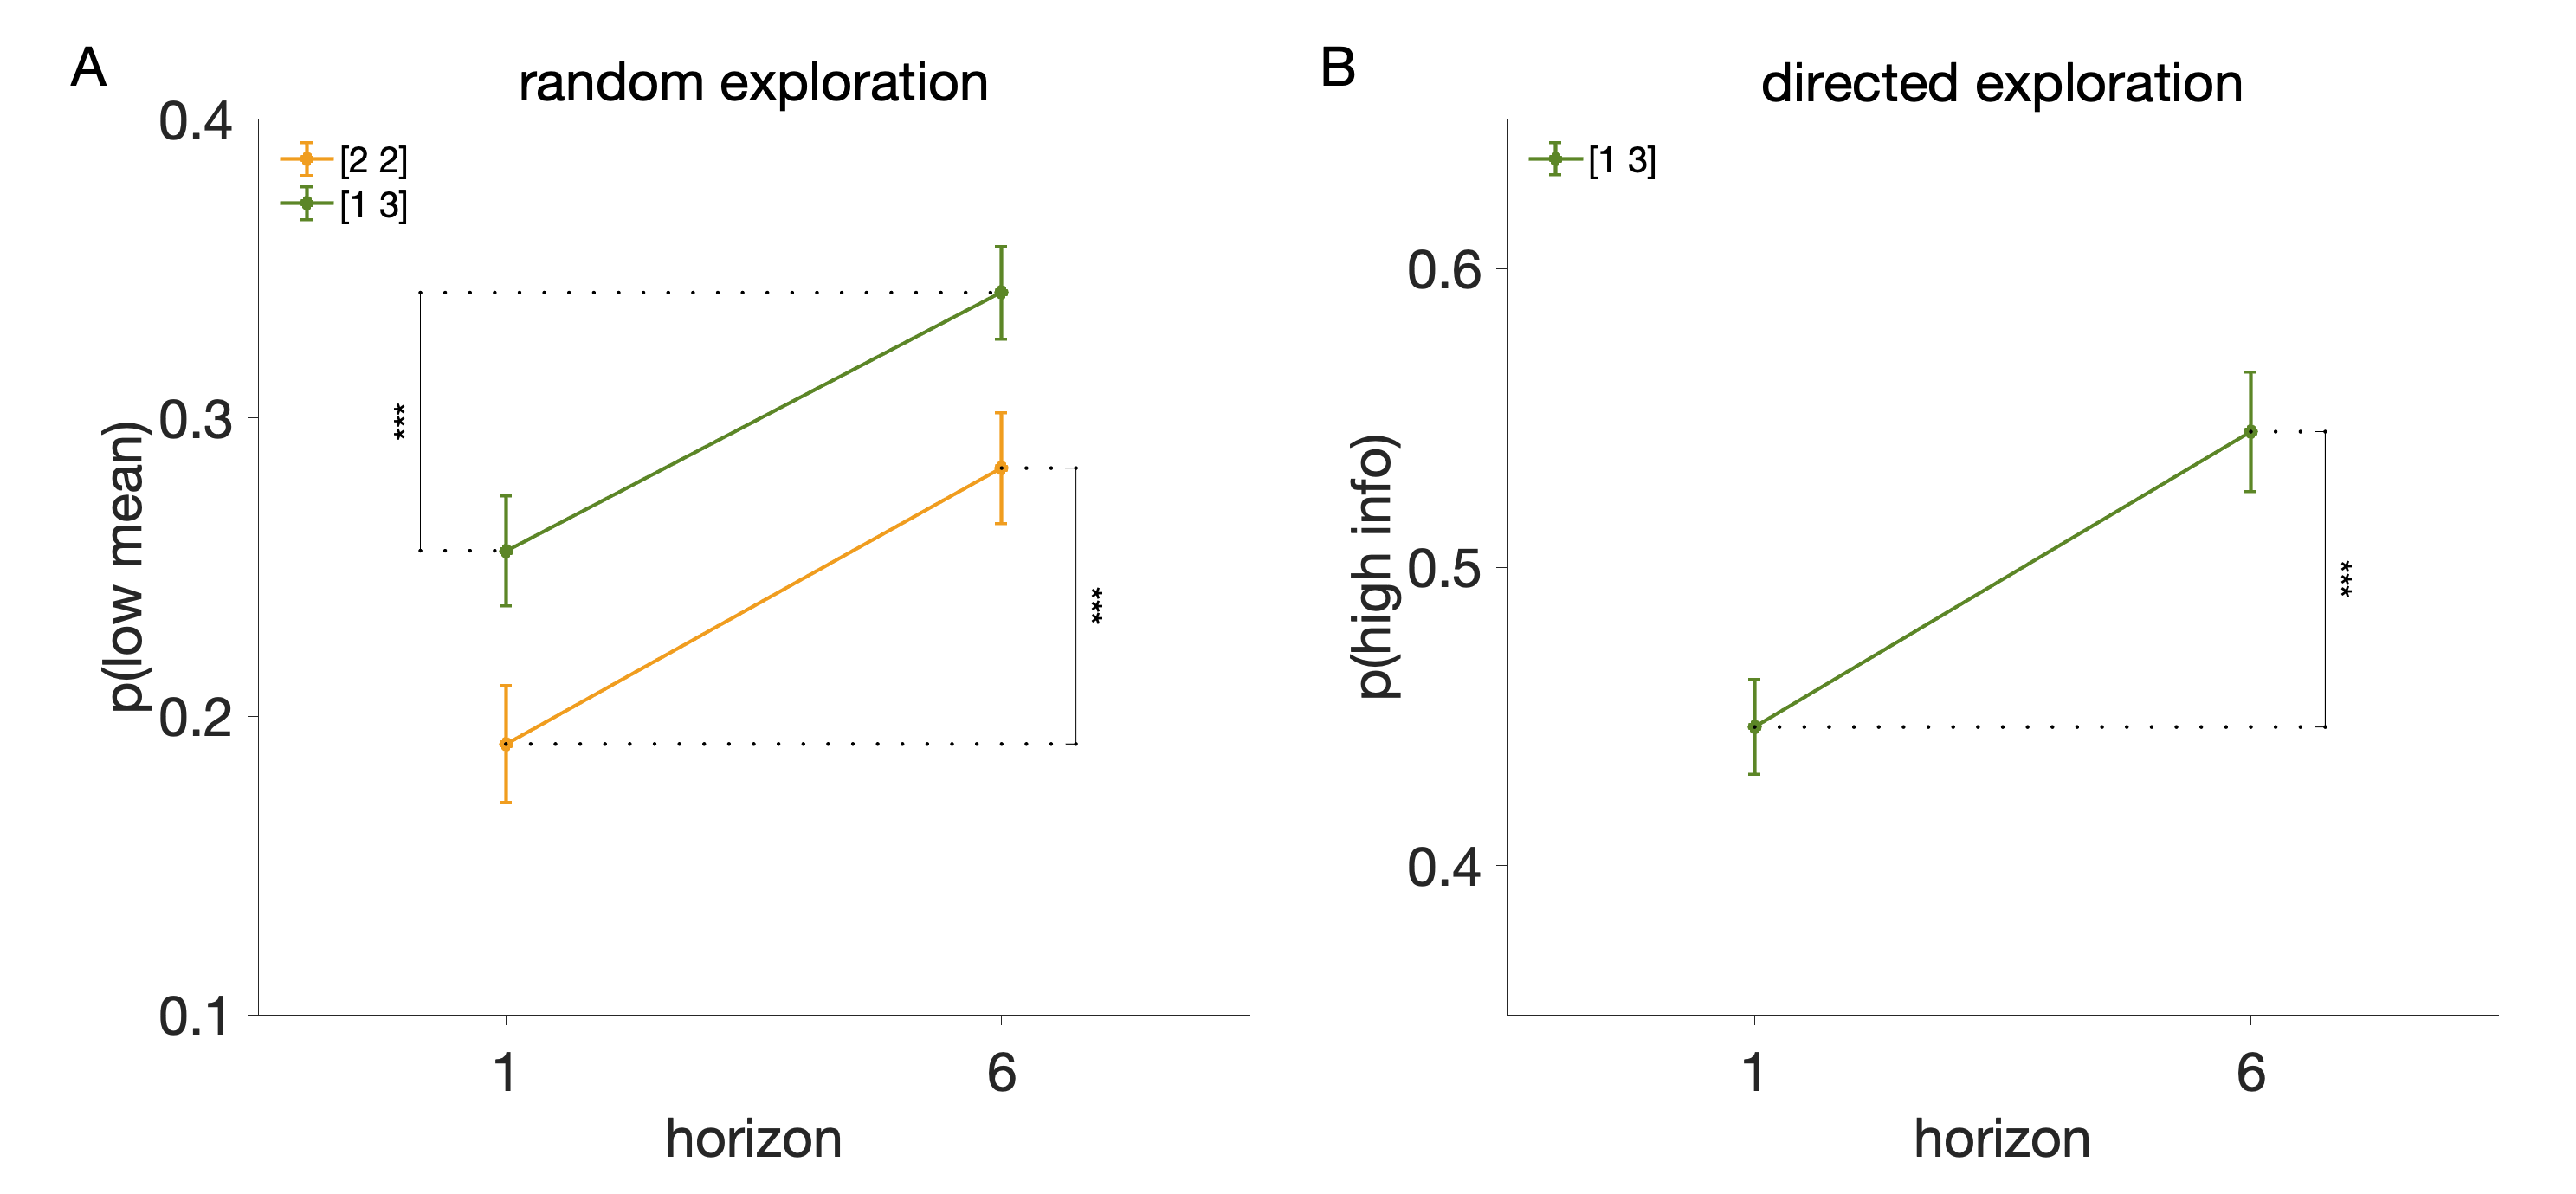
\includegraphics[width=\textwidth]{figures/RanDetNoise_modelfree_all.png}
			\caption{Replication of previous findings with data from all participants (i.e. no exclusions). Both  $p(\mbox{low mean})$ (A) and $p(\mbox{high info})$ (B) increase with horizon suggesting that people use both random and directed exploration in this task.  }
			\label{fig:modelfree2}
		\end{center}
	\end{figure}

	\begin{figure}[H]
		\begin{center}
			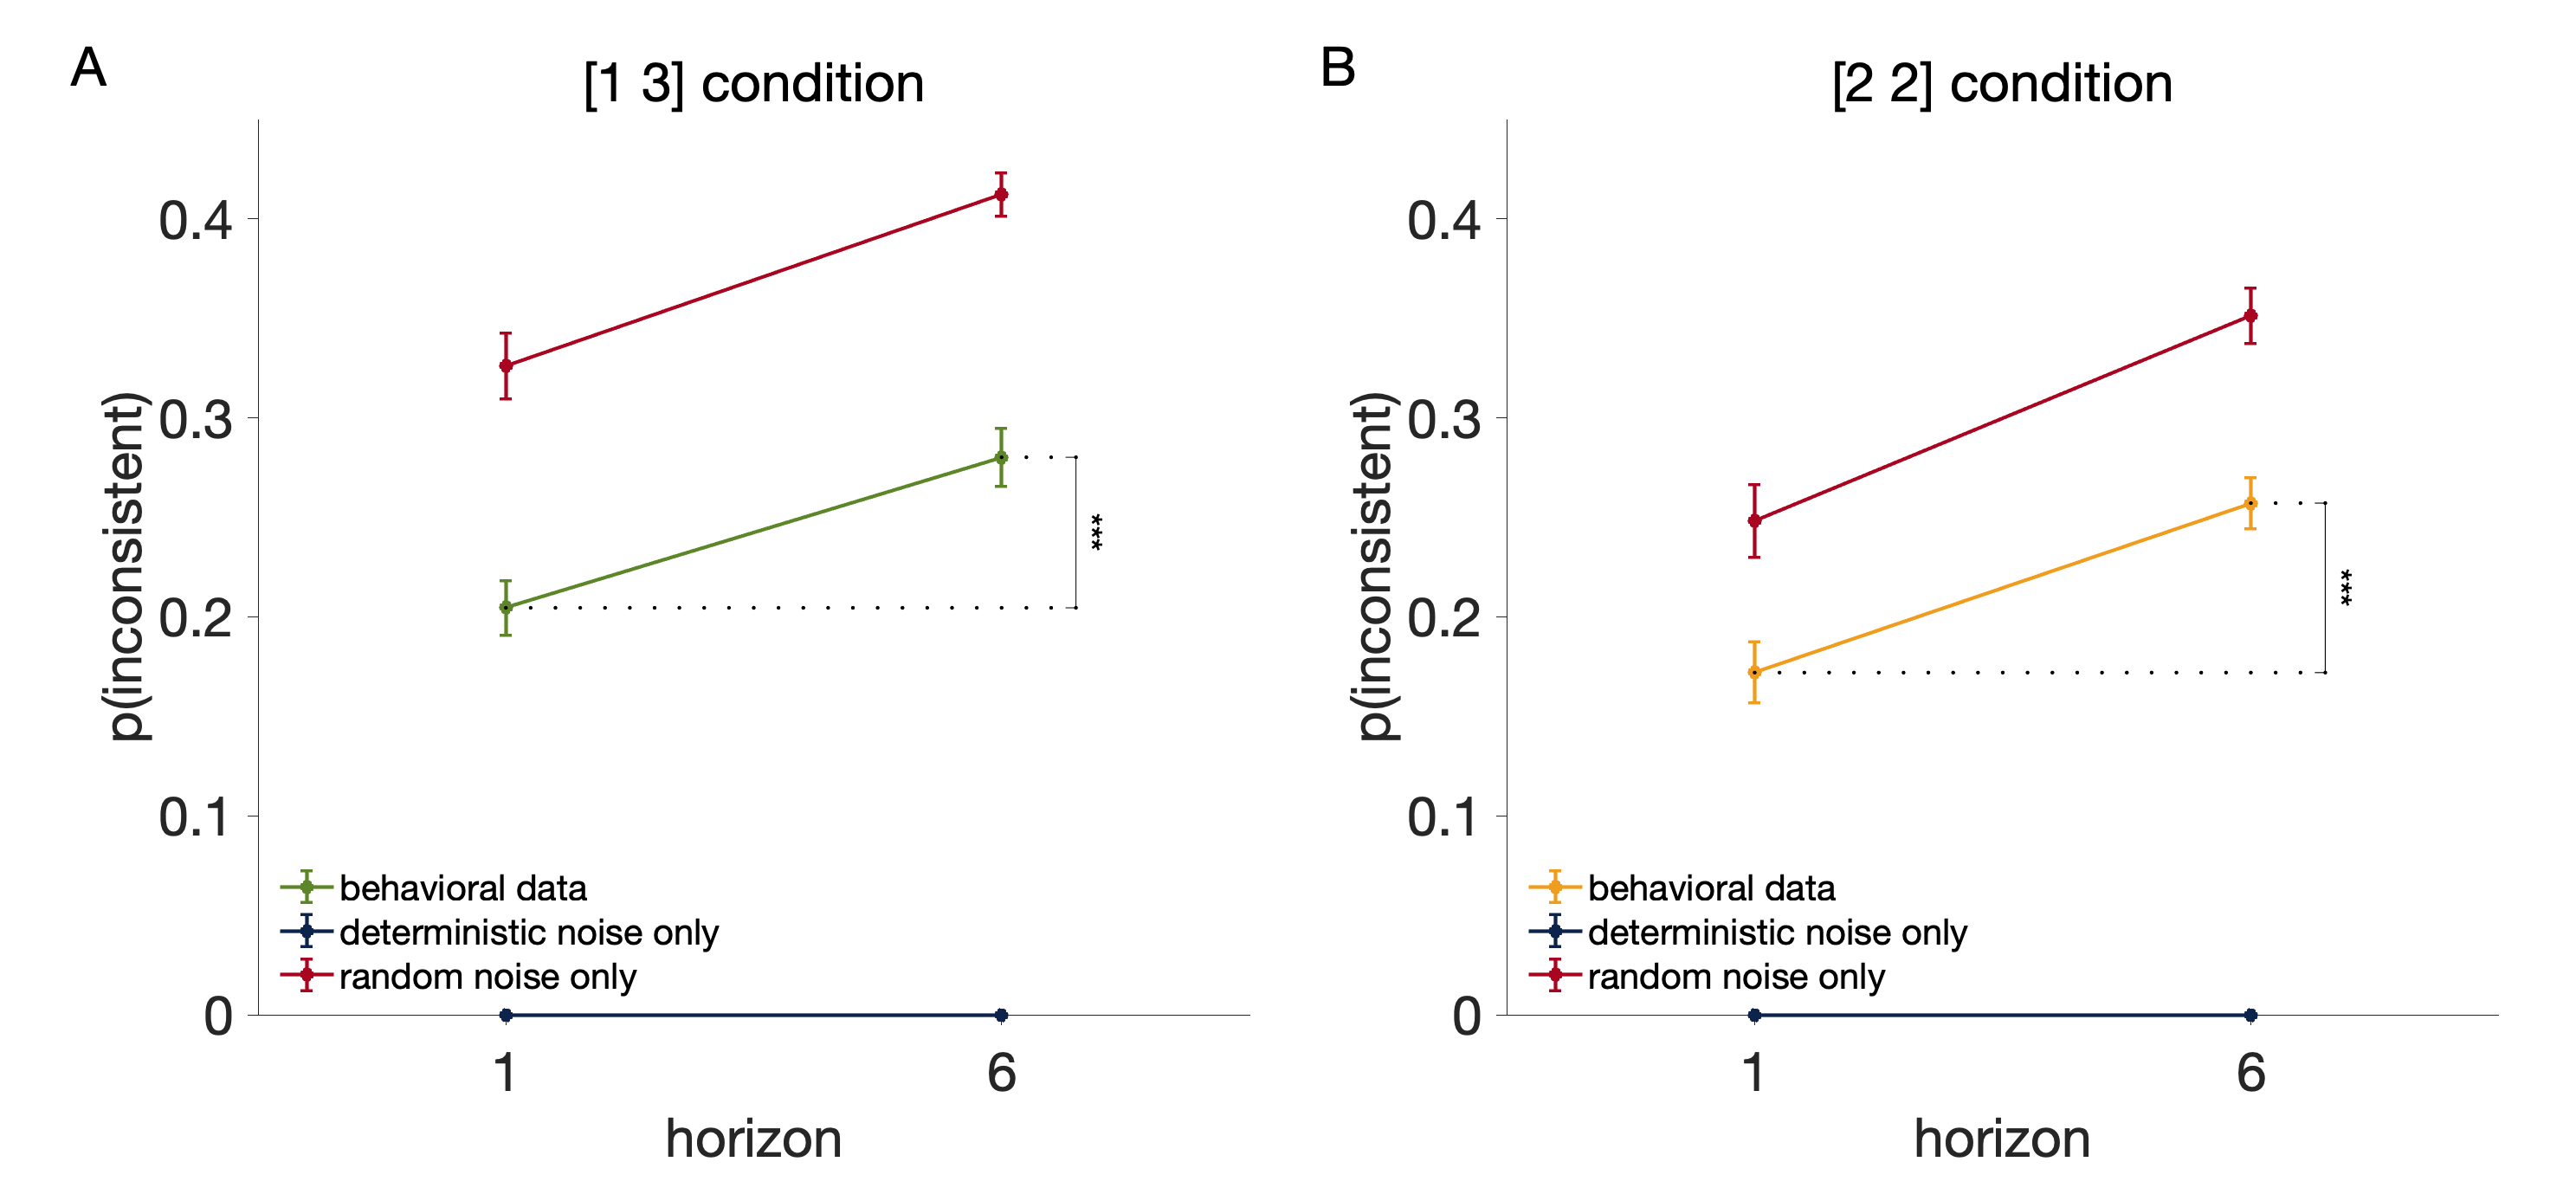
\includegraphics[width=\textwidth]{figures/RanDetNoise_2noise_all.png}
			\caption{Model-free analysis with data from all participants (i.e. no exclusions) suggests that both deterministic and random noise contribute to the choice variability in random exploration. For both the [1 3] (A) and [2 2] (B) condition, people show greater choice inconsistency in horizon 6 than horizon 1. However, the extent to which their choices are inconsistent lies between what is predicted by purely deterministic and random noise, suggesting that both noise sources influence the decision.}
			\label{fig:mf22}
		\end{center}
	\end{figure}
	\newpage
	\begin{figure}[H]
		\begin{center}
			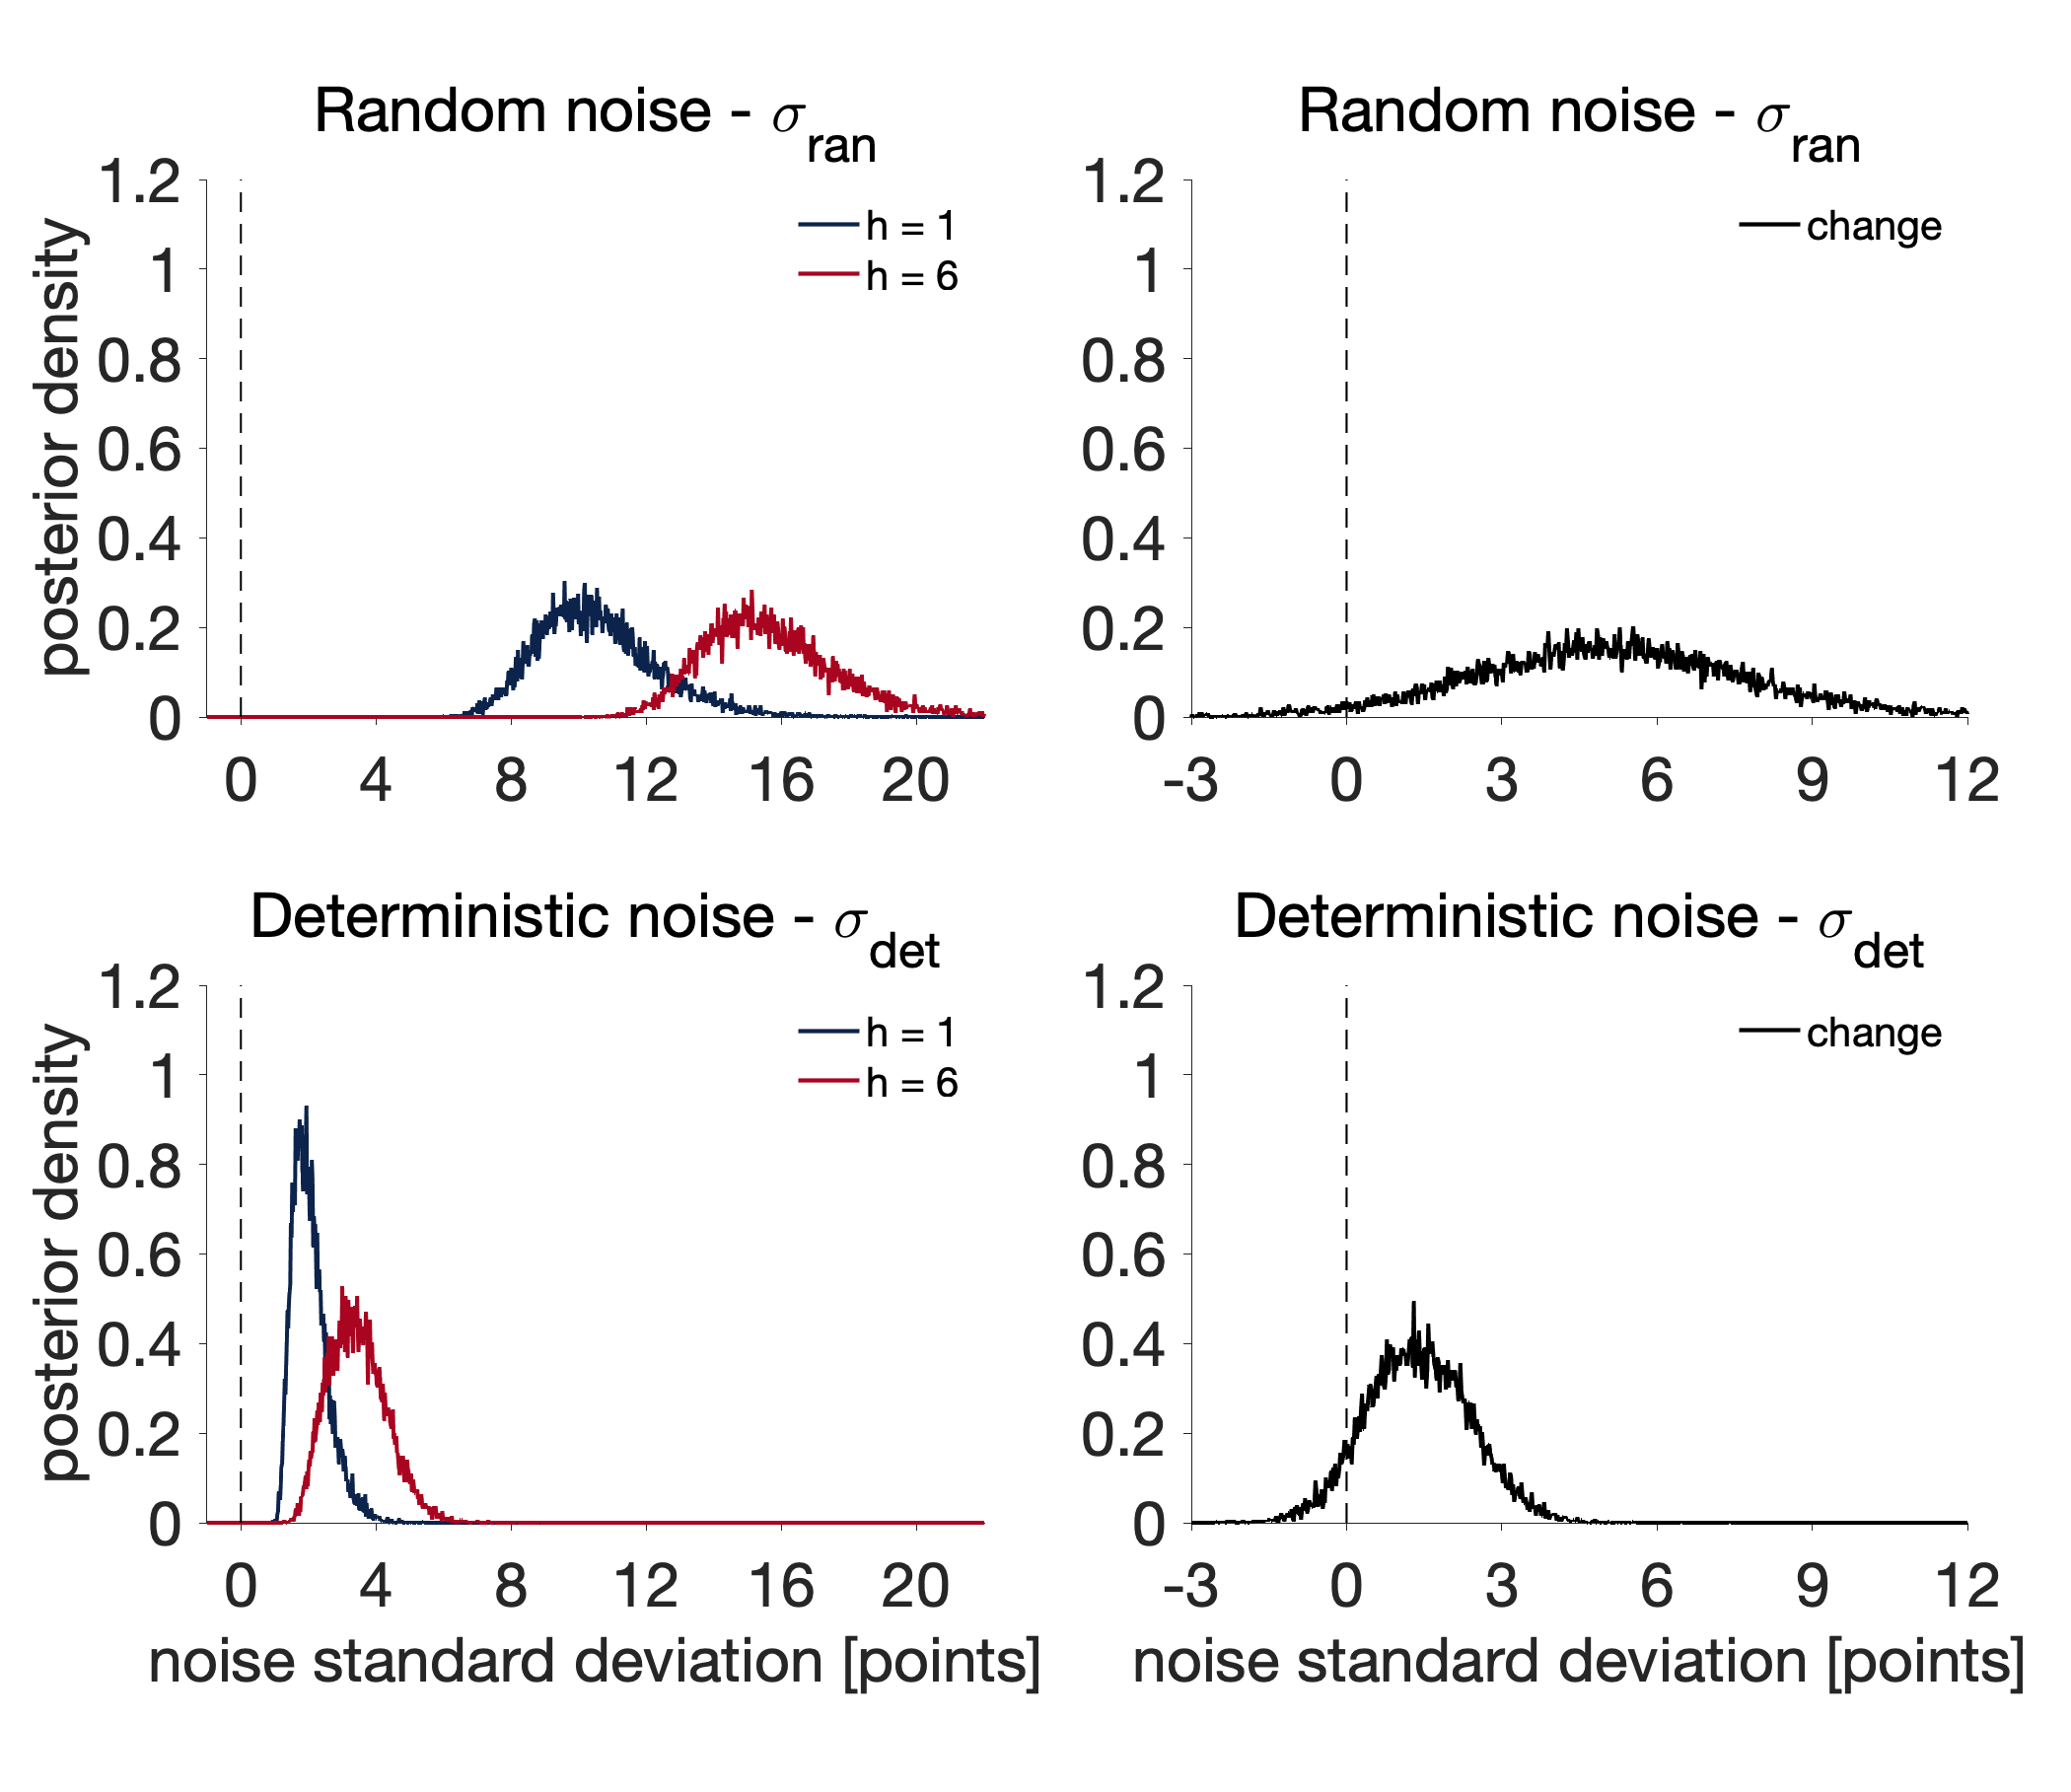
\includegraphics[width=1\textwidth]{figures/RanDetNoise_hyperprior_all.png}
			\caption{Model based analysis with data from all participants (i.e. no exclusions) showing the posterior distributions over the group-level mean of the standard deviations of  random and deterministic noise. Both random (A, B) and deterministic (C,D) noises are nonzero (A, C) and change with horizon (B, D).  However, random noise has both a greater magnitude overall (A, C) and a greater change with horizon (B, D) than deterministic noise.}
			%COMBINE FIGURES 4 AND 5, USE SEPARATE PANELS FOR EACH ONE, REMOVE INCORRECT RED SHADED REGION ON TOP PANEL OF FIGURE 5, Y-AXIS CAN BE LABELED 'posterior density' X-AXIS IS 'noise standard deviation [points]'
			\label{fig:mb12}
		\end{center}
	\end{figure}
	
	%\bibliographystyle{plainnat}
	%\bibliographystyle{unsrt}
	%\bibliography{Refs/refs}
	
	% add the Bibliography to the Table of Contents
	%\cleardoublepage
	%\ifdefined\phantomsection
	%\phantomsection  % makes hyperref recognize this section properly for pdf link
	%\else
	%\fi
	%\addcontentsline{toc}{chapter}{Bibliography}

\end{document}
